\documentclass[a4paper,11pt]{article}
\usepackage{amsmath,amsthm,amsfonts,amssymb,amscd,amstext,vmargin,graphics,graphicx,tabularx,multicol} 
\usepackage[francais]{babel}
\usepackage[utf8]{inputenc}  
\usepackage[T1]{fontenc} 
\usepackage{pstricks-add,tikz,tkz-tab,variations}
\usepackage[autolanguage,np]{numprint} 
\usepackage{yhmath}

\setmarginsrb{1.5cm}{0.5cm}{1cm}{0.5cm}{0cm}{0cm}{0cm}{0cm} %Gauche, haut, droite, haut
\newcounter{numexo}
\newcommand{\exo}[1]{\stepcounter{numexo}\noindent{\bf \underline{Exercice~\thenumexo}}}
\reversemarginpar


\newcounter{enumtabi}
\newcounter{enumtaba}
\newcommand{\q}{\stepcounter{enumtabi} \theenumtabi.  }
\newcommand{\qa}{\stepcounter{enumtaba} (\alph{enumtaba}) }
\newcommand{\initq}{\setcounter{enumtabi}{0}}
\newcommand{\initqa}{\setcounter{enumtaba}{0}}

\newcommand{\be}{\begin{enumerate}}
\newcommand{\ee}{\end{enumerate}}
\newcommand{\bi}{\begin{itemize}}
\newcommand{\ei}{\end{itemize}}
\newcommand{\bp}{\begin{pspicture*}}
\newcommand{\ep}{\end{pspicture*}}
\newcommand{\bt}{\begin{tabular}}
\newcommand{\et}{\end{tabular}}
\renewcommand{\tabularxcolumn}[1]{>{\centering}m{#1}} %(colonne m{} centrée, au lieu de p par défault) 
\newcommand{\tnl}{\tabularnewline}

\newcommand{\bmul}[1]{\begin{multicols}{#1}}
\newcommand{\emul}{\end{multicols}}

\newcommand{\trait}{\noindent \rule{\linewidth}{0.2mm}}
\newcommand{\hs}[1]{\hspace{#1}}
\newcommand{\vs}[1]{\vspace{#1}}

\newcommand{\N}{\mathbb{N}}
\newcommand{\Z}{\mathbb{Z}}
\newcommand{\R}{\mathbb{R}}
\newcommand{\C}{\mathbb{C}}
\newcommand{\Dcal}{\mathcal{D}}
\newcommand{\Ccal}{\mathcal{C}}
\newcommand{\mc}{\mathcal}

\newcommand{\vect}[1]{\overrightarrow{#1}}
\newcommand{\ds}{\displaystyle}
\newcommand{\eq}{\quad \Leftrightarrow \quad}
\newcommand{\vecti}{\vec{\imath}}
\newcommand{\vectj}{\vec{\jmath}}
\newcommand{\Oij}{(O;\vec{\imath}, \vec{\jmath})}
\newcommand{\OIJ}{(O;I,J)}




\newcommand{\reponse}[1][1]{%
\multido{}{#1}{\makebox[\linewidth]{\rule[0pt]{0pt}{20pt}\dotfill}
}}

\newcommand{\titre}[5] 
% #1: titre #2: haut gauche #3: bas gauche #4: haut droite #5: bas droite
{
\noindent #2 \hfill #4 \\
#3 \hfill #5

\vspace{-1.6cm}

\begin{center}\rule{6cm}{0.5mm}\end{center}
\vspace{0.2cm}
\begin{center}{\large{\textbf{#1}}}\end{center}
\begin{center}\rule{6cm}{0.5mm}\end{center}
}



\begin{document}
\pagestyle{empty}
\titre{Chapitre 9 : Symétrie axiale}{}{}{}{}

\vspace*{1cm}

\begin{center}
{\Large \textbf{Niveau 1 :}}
\end{center}

\vspace*{1cm}

$\rightarrow$ \textbf{Savoir reconnaître une symétrie axiale}\\

\vspace*{0.5cm}


\exo \\ Compléter la définition du symétrique d'une figure. \\

Lorsque deux figures se superposent par pliage suivant une droite, on dit que les deux figures sont . . . . . . . . . . . . . .  par rapport à cette droite.\\
Cette droite est alors appelée un . . . . . . de . . . . . . . . . . . .\\

\exo \\ Compléter la définition du symétrique d'un point par rapport à une droite.\\

Deux points E et E' sont symétriques par rapport à une droite (d) si la droite (d) est la . . . . . . . . . . . . . . . . . . . du segment [EE'].\\


\exo \\ Jules a essayé de reproduire le dessin de droite en recopiant son reflet à travers un miroir. Jules a presque réussi a dessiner le symétrique du dessin de droite, malheureusement, il a commis 7 erreurs.

Il faut l'aider à les retrouver ! Pour cibler où se trouve une erreur, citer les cases où elle se trouve.\\
 Exemple : la case B1.\\

\includegraphics[scale=1]{symétrie2.eps} \\

\noindent \reponse[3]\\



\exo \\ Compléter les phrases suivantes en observant la figure ci-dessous.\\

\includegraphics[scale=1]{symétrie3.eps} \\

\initqa \qa Le symétrique du point R par rapport à la droite (YE) est . . . . \\

\qa Le symétrique du point A par rapport à la droite (YE) est . . . . \\

\qa  Le symétrique du point I par rapport à la droite (YE) est . . . . \\

\exo \\ Compléter les phrases suivantes en observant la figure ci-dessous.\\

\includegraphics[scale=1]{symétrie4.eps} \\

\initqa \qa Le symétrique du point C par rapport à la droite (d) est le point . . . .\\

\qa Le symétrique du point D par rapport à la droite (d) est le point . . . .\\

\qa Le symétrique du point E par rapport à la droite (d) est le point . . . .\\



\exo \\ Les questions suivantes feront référence à la figure ci-dessous, où le polygone GHIJ est le symétrique du polygone CDEF par rapport à la droite (AB).\\
Cliquer sur la bonne réponse.\\

\begin{tabular}{|c|c|c|c|}
\hline 
La doite (AB) est la médiatrice du segment : & [EH] & [CH] & [FJ] \\ 
\hline 
Le symétrique du point E est le point :  & I & G & H \\ 
\hline 
Le symétrique du segment [ED] est :  & (IH) & ID & [IH] \\ 
\hline 
\end{tabular} 


\textbf{Remarque :} On pourrait ajouter des exercices de construction de symétrique sur les 5 nveaux.

\vspace*{1cm}

$\rightarrow$ \textbf{Axe de symétrie}\\

\vspace*{0.5cm}



\exo \\ Quelle est l'axe de symétrie de la figure ci-dessous ?\\

\includegraphics[scale=1]{symétrie3.eps} \\

\noindent \reponse[1]\\



\exo \\ Dans la figure ci-dessous, dire si les droites (d) et (d') sont ou ne sont pas des axes de symétrie.\\


\includegraphics[scale=1.1]{axe1.eps}  \\

Réponse :\\ 

La droite (d) : . . . \\

La droite (d') : . . . \\



\textbf{Remarque :} On pourrait ajouter des exercices de construction d'axe de symétrie sur les 5 nveaux.

\vspace*{1cm}

$\rightarrow$ \textbf{Exercices de démonstration sur les propriétés}\\

\vspace*{0.5cm}



\exo \\ Compléter la propriété sur le symétrique d'une droite par rapport à une droite.\\

Le symétrique d'une droite (d) par rapport à une droite ($\Delta$) est . . . . . . . . . . . .\\

\exo \\ Compléter la propriété sur le symétrique d'un segment par rapport à une droite.\\

Le symétrique d'un segment par rapport à une droite ($\Delta$) est . . . . . . . . . . . . . . de même . . . . . . . . .\\

\exo \\ Compléter la propriété sur le symétrique d'un cercle par rapport à une droite.\\

Le symétrique d'un cercle par rapport à une droite ($\Delta$) est . . . . . . . . . . . . . .  de même . . . . . . . . .\\


\exo \\ Les deux figures ci-dessous sont symétriques par rapport à la droite (d).\\

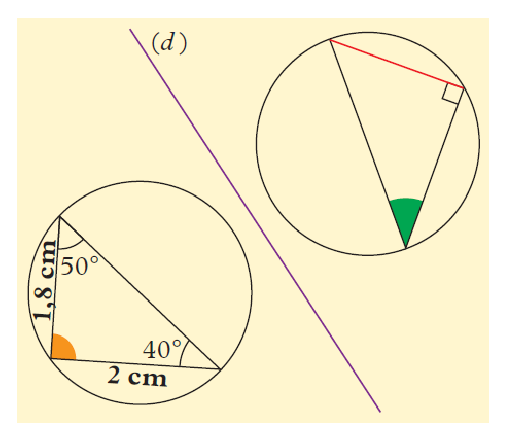
\includegraphics[scale=1]{prop3.eps} \\

\initqa \qa Combien mesure l'angle orange ? . . . \\

\qa Combien mesure l'angle vert ? . . . \\

\qa Quelle est la longueur du segment rouge ? . . .\\


\vspace*{0.5cm}

\begin{center}
{\Large \textbf{Niveau 2 :}}
\end{center}

\vspace*{1cm}

$\rightarrow$ \textbf{Savoir reconnaître une symétrie axiale}\\

\vspace*{0.5cm}


\exo \\ Compléter les phrases suivantes en observant la figure ci-dessous.\\

\includegraphics[scale=1]{symétrie5.eps} \\

\initqa \qa Le symétrique du point C par rapport à la droite (d) est le point . . . .\\

\qa Le symétrique du point D par rapport à la droite (d) est le point . . . .\\

\qa Le symétrique du point E par rapport à la droite (d) est le point . . . .\\


\exo \\ Compléter les phrases suivantes en observant la figure ci-dessous.\\

\includegraphics[scale=1]{symétrie3.eps} \\

\initqa \qa Le symétrique du segment [RT] par rapport à la droite (YE) est . . . . \\

\qa Le symétrique du segment [YZ] par rapport à la droite (YE) est . . . . \\

\qa  Le symétrique du segment [AT] par rapport à la droite (YE) est . . . . \\




\exo \\ On donne la figure suivante :\\

\includegraphics[scale=1]{symétrie6.eps} \\

Quelle est la couleur du symétrique de la flèche noire par rapport à la droite (d) ?\\

Réponse : . . . . . . . . . . . . . . . .\\


\exo \\ \\ Répondre aux questions suivantes en observant la figure ci-dessous.\\

\includegraphics[scale=1.1]{symétrie10.eps} \\

\initqa \qa Quel est le symétrique du point A par rapport à la droite (OA) ? Réponse : . . . . .\\

\qa Quel est le symétrique du point B' par rapport à la droite (OA) ? Réponse : . . . . .\\

\qa Quel est le symétrique du point A' par rapport à la droite (OA) ? Réponse : . . . . .\\

\qa Quel est le symétrique du point H par rapport à la droite (OA) ? Réponse : . . . . .\\



\vspace*{1cm}

$\rightarrow$ \textbf{Axe de symétrie}\\

\vspace*{0.5cm}



\exo \\ Dans la figure ci-dessous, dire si les droites (d) et (d') sont ou ne sont pas des axes de symétrie.\\


\includegraphics[scale=1.1]{axe2.eps}  \\

Réponse :\\ 

La droite (d) : . . . \\

La droite (d') : . . . \\

\exo \\ Dans la figure ci-dessous, dire si les droites (d) et (d') sont ou ne sont pas des axes de symétrie.\\


\includegraphics[scale=1.1]{axe3.eps}  \\

Réponse :\\ 

La droite (d) : . . . \\

La droite (d') : . . . \\

\exo \\ Compléter les phrases suivantes en observant la figure ci-dessous.\\

\includegraphics[scale=1]{axe4.eps} \\

\initqa \qa La figure rouge est le symétrique de la figure bleue par rapport à la droite . . . . .\\

\qa La figure verte est le symétrique de la figure bleue par rapport à la droite . . . . .\\


\vspace*{1cm}

$\rightarrow$ \textbf{Exercices de démonstration sur les propriétés}\\

\vspace*{0.5cm}

\exo \\ Les deux figures ci-dessous sont symétriques par rapport à la droite (d).\\

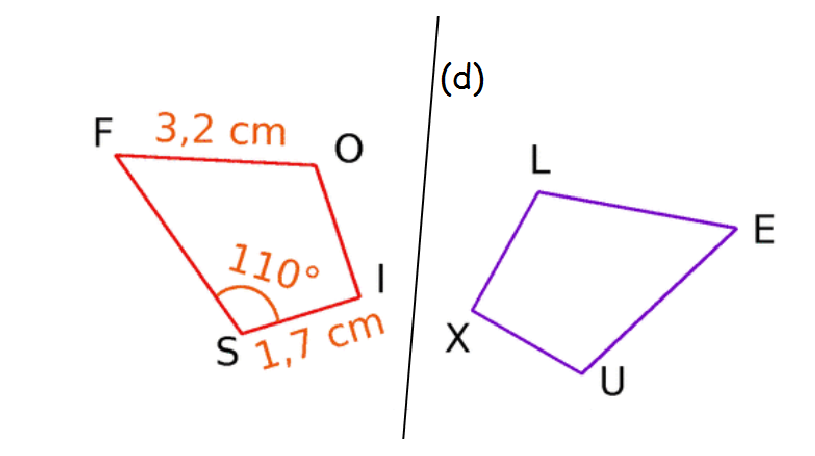
\includegraphics[scale=1]{prop1.eps} \\

\initqa \qa Quel est le symétrique du segment [LE] ? . . . . . . . . . . . . . . . . .\\

\qa Citer parmi les propriétés ci-dessous, celle qui nous permet de connaître la longueur du segment [LE]. \\


\includegraphics[scale=0.6]{prop1a.eps} \includegraphics[scale=0.6]{prop1c.eps}\\

\includegraphics[scale=0.6]{prop1b.eps}  \includegraphics[scale=0.6]{prop1d.eps} \\

Réponse : . . . . . . . . . . . . . . . .\\

\qa Quelle est donc la longueur du segment [LE] ? . . . . . . . . . . . . . . . . . . .\\





\exo \\ Les deux figures ci-dessous sont symétriques par rapport à la droite (d).\\

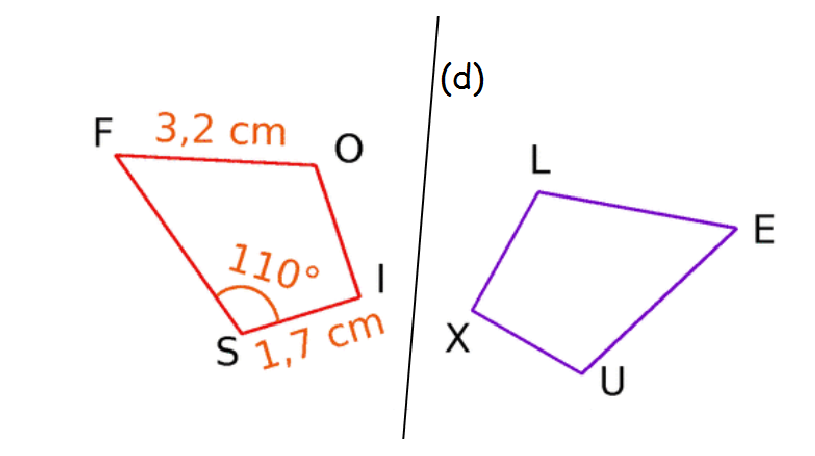
\includegraphics[scale=1]{prop1.eps} \\

\initqa \qa Quel est le symétrique du segment [XU] ? . . . . . . . . . . . . . . . . .\\

\qa Citer parmi les propriétés ci-dessous, celle qui nous permet de connaître la longueur du segment [XU]. \\


\includegraphics[scale=0.6]{prop1a.eps} \includegraphics[scale=0.6]{prop1c.eps}\\

\includegraphics[scale=0.6]{prop1b.eps}  \includegraphics[scale=0.6]{prop1d.eps} \\

Réponse : . . . . . . . . . . . . . . . .\\

\qa Quelle est donc la longueur du segment [XU] ? . . . . . . . . . . . . . . . . . . .\\

















\begin{center}
{\Large \textbf{Niveau 3 :}}
\end{center}

\vspace*{1cm}

$\rightarrow$ \textbf{Savoir reconnaître une symétrie axiale}\\

\vspace*{0.5cm}





\exo \\ Compléter les phrases suivantes en observant la figure ci-dessous.\\

\includegraphics[scale=1]{symétrie3.eps} \\

\initqa \qa Le symétrique du segment [ZE] par rapport à la droite (YE) est . . . . \\

\qa Le symétrique de la droite (IT) par rapport à la droite (YE) est . . . . \\

\qa  Le symétrique de la droite (YI) par rapport à la droite (YE) est . . . . \\



\exo \\ Compléter les phrases suivantes en observant la figure ci-dessous.\\

\includegraphics[scale=1]{symétrie3.eps} \\

\initqa \qa Le symétrique de l'arc de cercle $\wideparen{ER}$  par rapport à la droite (YE) est . . . . \\

\qa Le symétrique du triangle RYT par rapport à la droite (YE) est . . . . \\

\qa  Le symétrique du triangle ZRY par rapport à la droite (YE) est . . . . \\


\exo \\ Compléter les phrases suivantes en observant la figure ci-dessous.\\

\includegraphics[scale=1]{symétrie7.eps} \\


\initqa \qa Le symétrique du carré noir par rapport à la droite $(d_{1})$ est le carré  . . . . \\


 \qa Le symétrique du carré noir par rapport à la droite $(d_{2})$ est le carré  . . . . \\
 
  \qa Le symétrique du carré noir par rapport à la droite $(d_{3})$ est le carré  . . . . \\


\exo \\ \\ Répondre aux questions suivantes en observant la figure ci-dessous.\\

\includegraphics[scale=1.1]{symétrie10.eps} \\

\initqa \qa Quel est le symétrique du segment [AB'] par rapport à la droite (OA) ? Réponse : . . . . .\\

\qa Quel est le symétrique du segment [H'A]  par rapport à la droite (OA) ? Réponse : . . . . .\\

\qa Quel est le symétrique de la droite (BF) par rapport à la droite (OA) ? Réponse : . . . . .\\




\vspace*{1cm}

$\rightarrow$ \textbf{Axe de symétrie}\\

\vspace*{0.5cm}




\exo \\ Compléter les phrases suivantes en observant la figure ci-dessous.\\

\includegraphics[scale=1]{symétrie7.eps} \\


\initqa \qa Le symétrique du carré noir par rapport à la droite . . . . est le carré  vert. \\


 \qa Le symétrique du carré rouge par rapport à la droite . . . . est le carré  noir. \\
 
  \qa Le symétrique du carré bleu par rapport à la droite . . . . est le carré  noir.\\


\exo \\ Combien d'axe de symétrie la figure ci-dessous possède-t-elle ?\\

\includegraphics[scale=1]{symétrie10.eps} \\

Réponse : . . . .\\



\vspace*{1cm}

$\rightarrow$ \textbf{Exercices de démonstration sur les propriétés}\\

\vspace*{0.5cm}





\exo \\ Les deux figures ci-dessous sont symétriques par rapport à la droite (d).\\

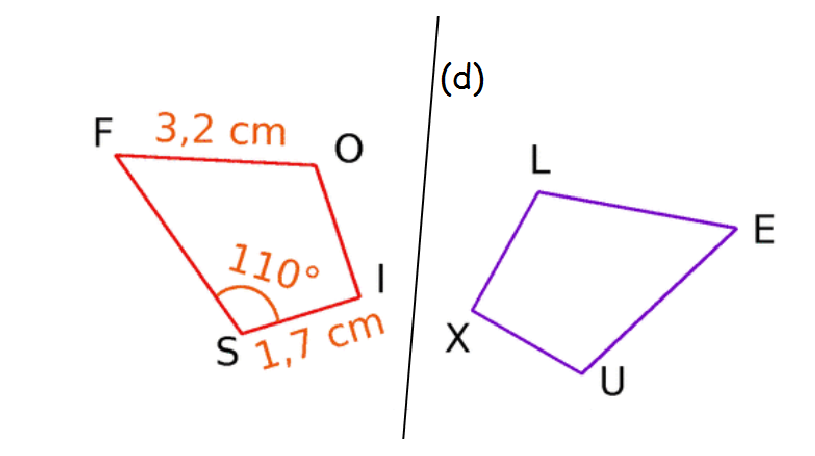
\includegraphics[scale=1]{prop1.eps} \\

\initqa \qa Quel est le symétrique de l'angle $\widehat{XUE}$ ? . . . . . . . . . . . . . . . . .\\

\qa Citer parmi les propriétés ci-dessous, celle qui nous permet de connaître la mesure de l'angle $\widehat{XUE}$ . \\


\includegraphics[scale=0.6]{prop1a.eps} \includegraphics[scale=0.6]{prop1c.eps}\\

\includegraphics[scale=0.6]{prop1b.eps}  \includegraphics[scale=0.6]{prop1d.eps} \\

Réponse : . . . . . . . . . . . . . . . .\\

\qa Quelle est donc la mesure de l'angle $\widehat{XUE}$  ? . . . . . . . . . . . . . . . . . . .\\


\exo \\ Les deux figures ci-dessous sont symétriques par rapport à la droite (d).\\


\includegraphics[scale=1]{prop4.eps}\\

Quelle est la nature du triangle TMP ?\\
\reponse[2]\\

\begin{center}
{\Large \textbf{Niveau 4:}}
\end{center}

\vspace*{1cm}

$\rightarrow$ \textbf{Savoir reconnaître une symétrie axiale}\\

\vspace*{0.5cm}




\exo \\ Compléter les phrases suivantes en observant la figure ci-dessous.\\

\includegraphics[scale=1]{symétrie3.eps} \\

\initqa \qa Le symétrique du demi-cercle $\wideparen{ZR}$ par rapport à la droite (YE) est . . . . \\

\qa Le symétrique du quadrilatère AZIY par rapport à la droite (YE) est . . . . \\

\qa  Le symétrique du polygone TYZR par rapport à la droite (YE) est . . . . \\


\exo \\  On donne la figure suivante :\\

\includegraphics[scale=1.1]{symétrie10.eps} \\

En considérant la symétrie d'axe (OH), compléter le tableau suivant :\\

\begin{tabular}{|c|c|c|c|c|c|}
\hline 
Le symétrique de .... &  A & B' & [AB'] & H & [A'H] \\ 
\hline 
par rapport à la droite (OH) est ... & . . .  & . . . & . . . & . . . & . . . \\ 
\hline 
\end{tabular} 

\exo \\  On donne la figure suivante :\\

\includegraphics[scale=1.1]{symétrie10.eps} \\

En considérant la symétrie d'axe (OB), compléter le tableau suivant :\\

\begin{tabular}{|c|c|c|c|c|c|}
\hline 
Le symétrique de .... &  A & B' & [AB'] & H & [A'H] \\ 
\hline 
par rapport à la droite (OB) est ... & . . .  & . . . & . . . & . . . & . . . \\ 
\hline 
\end{tabular} 


\exo \\  Compléter les phrases suivantes en observant la figure ci-dessous.\\

\includegraphics[scale=1]{symétrie12.eps} \\

\initqa \qa Le symétrique du triangle 3 par rapport à la droite (PH) est  le triangle . . . \\

\qa Le symétrique du triangle 10 par rapport à la droite (KE) est  le triangle . . . \\

\qa Le symétrique du triangle 6 par rapport à la droite (ME) est  le triangle . . . \\

\qa Le symétrique du triangle 11 par rapport à la droite (CK) est  le triangle . . . \\



\vspace*{1cm}

$\rightarrow$ \textbf{Axe de symétrie}\\

\vspace*{0.5cm}


\exo \\ Citer tous les axes de symétrie de la figure ci-dessous.\\

\includegraphics[scale=1]{symétrie10.eps} \\



\exo \\  Compléter les phrases suivantes en observant la figure ci-dessous.\\

\includegraphics[scale=1]{symétrie12.eps} \\

\initqa \qa Le symétrique du triangle 2 par rapport à la droite . . . . est  le triangle 9. \\

\qa Le symétrique du triangle 8 par rapport à la droite . . . . est  le triangle 17. \\

\qa Le symétrique du triangle 5 par rapport à la droite . . . . est  le triangle 14. \\

\exo \\ Voici une série de panneaux du code de la route :\\

\includegraphics[scale=1.2]{axe6.eps} \\

Chaque ligne correspond à un panneau, cliquer sur le nombre d'axe de symétrie qu'il possède.\\

\begin{tabular}{|c|p{2.5cm}|p{2.5cm}|p{2.5cm}|p{2.5cm}|}
\hline 
 & \multicolumn{4}{|c|}{Nombre d'axe de symétrie} \\ 
\hline 
Panneau 1 & 0 & 1 & 2 & plus de 2 \\ 
\hline 
Panneau 2 & 0 & 1 & 2 & plus de 2 \\  
\hline 
Panneau 3 & 0 & 1 & 2 & plus de 2 \\ 
\hline 
Panneau 4 & 0 & 1 & 2 & plus de 2 \\ 
\hline 
Panneau 5 & 0 & 1 & 2 & plus de 2 \\ 
\hline 
\end{tabular} 

\exo \\ Voici une série de lettre de l'alphabet :\\

\includegraphics[scale=0.6]{symétrie14.eps} \\

Chaque ligne correspond à une lettre, cliquer sur le nombre d'axe de symétrie qu'elle possède.\\

\begin{tabular}{|c|p{2.5cm}|p{2.5cm}|p{2.5cm}|p{2.5cm}|}
\hline 
 & \multicolumn{4}{|c|}{Nombre d'axe de symétrie} \\ 
\hline 
A & 0 & 1 & 2 & 3 \\ 
\hline 
B & 0 & 1 & 2 & 3 \\  
\hline 
D & 0 & 1 & 2 & 3 \\ 
\hline 
E & 0 & 1 & 2 & 3 \\ 
\hline 
H & 0 & 1 & 2 & 3 \\ 
\hline 
I & 0 & 1 & 2 & 3 \\ 
\hline 
J & 0 & 1 & 2 & 3 \\ 
\hline 
M & 0 & 1 & 2 & 3 \\ 
\hline 
N & 0 & 1 & 2 & 3 \\ 
\hline 
O & 0 & 1 & 2 & 3 \\ 
\hline 
\end{tabular} 


\vspace*{1cm}

$\rightarrow$ \textbf{Exercices de démonstration sur les propriétés}\\

\vspace*{0.5cm}










\exo \\ Les deux figures ci-dessous sont symétriques par rapport à la droite (d).\\

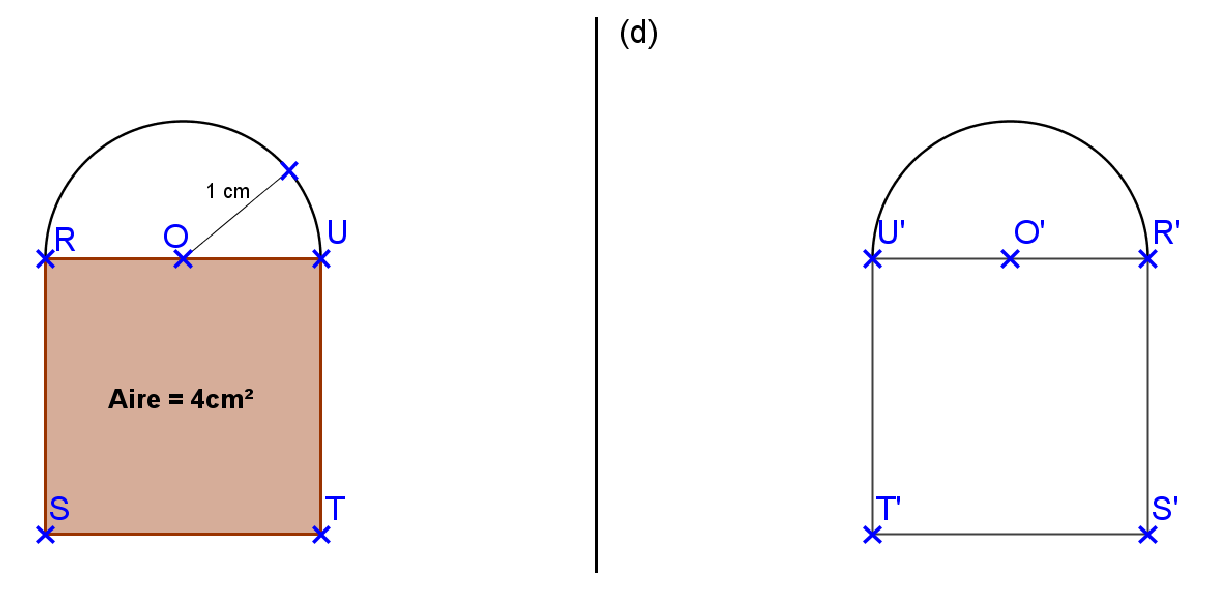
\includegraphics[scale=0.8]{prop2.eps} \\

\initqa \qa Citer parmi les propriétés ci-dessous, celle qui nous permet de connaître la mesure du rayon du cercle de centre O' passant par le point U'. \\


\includegraphics[scale=0.6]{prop1a.eps} \includegraphics[scale=0.6]{prop1c.eps}\\

\includegraphics[scale=0.6]{prop1b.eps}  \includegraphics[scale=0.6]{prop1d.eps} \\

Réponse : . . . . . . . . . . . . . . . .\\

\qa Quelle est donc la mesure du rayon du cercle de centre O' passant par le point U' ? . . . . . . . . . . . . . . . . . . .\\


\exo \\ Les deux figures ci-dessous sont symétriques par rapport à la droite (d).\\

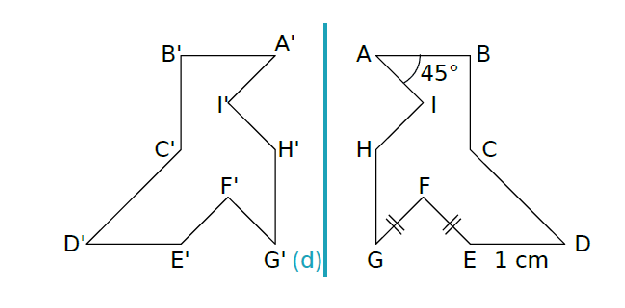
\includegraphics[scale=0.85]{interro7.eps} 


On souhaite trouver la mesure du segment[D'E'], compléter la démonstration suivante :\\

Les segments [D'E'] et . . . . . sont symétriques par rapport à la droite (d).\\
Or : AE = . . . . .\\
Donc : D'E' = . . . . .\\




\exo \\ Les deux figures ci-dessous sont symétriques par rapport à la droite (d).\\


\includegraphics[scale=1]{prop4.eps}\\

On souhaite trouver la mesure du segment[MT], compléter la démonstration suivante :\\

Les segments [MT] et . . . . . sont symétriques par rapport à la droite (d).\\
Or : EC = . . . . .\\
Donc : MT = . . . . .\\


\exo \\ Les deux figures ci-dessous sont symétriques par rapport à la droite (d).\\


\includegraphics[scale=1]{prop4.eps}\\

Que peut-on dire du point S ?\\
\reponse[2]\\

\begin{center}
{\Large \textbf{Niveau 5 :}}
\end{center}



\vspace*{1cm}

$\rightarrow$ \textbf{Savoir reconnaître une symétrie axiale}\\

\vspace*{0.5cm}

\exo \\ Dans la figure suivante, ABCD est un carré. On rappellera que les diagonales d'un carré se coupent en leur milieu.\\

\includegraphics[scale=1]{symétrie9.eps} \\


En considérant la symétrie d'axe (HF), compléter le tableau suivant :\\

\begin{tabular}{|c|c|c|c|c|c|}
\hline 
Le symétrique de .... & A & [EF] & (AC) & HEC & IDA \\ 
\hline 
par rapport à la droite (HF) est ... & . . . & . . . & . . . & . . . & . . . \\ 
\hline 
\end{tabular} 


\exo \\ Dans la figure suivante, ABCD est un carré. On rappellera que les diagonales d'un carré se coupent en leur milieu.\\

\includegraphics[scale=1]{symétrie9.eps} \\


En considérant la symétrie d'axe (AC), compléter le tableau suivant :\\

\begin{tabular}{|c|c|c|c|c|c|}
\hline 
Le symétrique de .... &  . . .& (DC) & . . . & (BD) & EFGD \\ 
\hline 
par rapport à la droite (AC) est ... & D & . . . & [EC] & . . . & . . . \\ 
\hline 
\end{tabular} 




\exo \\  Compléter les phrases suivantes en observant la figure ci-dessous.\\

\includegraphics[scale=1.2]{symétrie8.eps} \\

\initqa \qa Le symétrique du triangle 11 par rapport à la droite bleue est le triangle . . .\\

 \qa Le symétrique du triangle 18 par rapport à la droite en pointillés bleus est le triangle . . .\\

\qa Le symétrique du triangle 15 par rapport à la droite en pointillés rouges est le triangle . . .\\

\qa Le symétrique du triangle 3 par rapport à la droite verte est le triangle . . .\\





\exo \\ On donne la figure suivante :\\

\includegraphics[scale=1.2]{symétrie13.eps} \\

En remplaçant chaque lettre par son symétrique par rapport à la droite (d), vous pourrez décoder la phrase ci-dessous.\\

"YSE ZOFVE Q'SEF Y'O HWS" : . . . . . . . . . . . . . . . . . . . .\\


\vspace*{1cm}

$\rightarrow$ \textbf{Axe de symétrie}\\

\vspace*{0.5cm}


\exo \\  Compléter les phrases suivantes en observant la figure ci-dessous.\\

\includegraphics[scale=1.2]{symétrie8.eps} \\

\initqa \qa Le symétrique du triangle 1 par rapport à la droite . . . . . . . . . . .. est le triangle 16.\\

 \qa Le symétrique du triangle 13 par rapport à la droite . . . . . . . . . . . est le triangle 7.\\

\qa Le symétrique du triangle 4 par rapport à la droite . . . . . . . . . . . . . . est le triangle 5.\\

\qa Le symétrique du triangle 6 par rapport à la droite . . . . . . . . . . . . . . .  est le triangle 14.\\



\exo \\ Voici une série de panneaux du code de la route :\\

\includegraphics[scale=1.2]{axe5.eps} \\

Chaque ligne correspond à un panneau, cliquer sur le nombre d'axe de symétrie qu'il possède.\\

\begin{tabular}{|c|p{2.5cm}|p{2.5cm}|p{2.5cm}|p{2.5cm}|}
\hline 
 & \multicolumn{4}{|c|}{Nombre d'axe de symétrie} \\ 
\hline 
Panneau 1 & 0 & 1 & 2 & 3 \\ 
\hline 
Panneau 2 & 0 & 1 & 2 & 3 \\  
\hline 
Panneau 3 & 0 & 1 & 2 & 3 \\ 
\hline 
Panneau 4 & 0 & 1 & 2 & 3 \\ 
\hline 
Panneau 5 & 0 & 1 & 2 & 3 \\ 
\hline 
Panneau 6 & 0 & 1 & 2 & 3 \\ 
\hline 
Panneau 7 & 0 & 1 & 2 & 3 \\ 
\hline 
Panneau 8 & 0 & 1 & 2 & 3 \\ 
\hline 
Panneau 9 & 0 & 1 & 2 & 3 \\ 
\hline 
Panneau 10 & 0 & 1 & 2 & 3 \\ 
\hline 
\end{tabular} 





\vspace*{1cm}

$\rightarrow$ \textbf{Exercices de démonstration sur les propriétés}\\

\vspace*{0.5cm}



\exo \\ Les deux figures ci-dessous sont symétriques par rapport à la droite (d).\\

\includegraphics[scale=0.8]{prop2.eps} \\

\initqa  Citer parmi les propriétés ci-dessous, celle qui nous permet de connaître l'aire du polygone U'R'S'T'. \\


\includegraphics[scale=0.6]{prop1a.eps} \includegraphics[scale=0.6]{prop1c.eps}\\

\includegraphics[scale=0.6]{prop1b.eps}  \includegraphics[scale=0.6]{prop1d.eps} \\

Réponse : . . . . . . . . . . . . . . . .\\

\qa Quelle est donc l'aire du polygone U'R'S'T'  ? . . . . . . . . . . . . . . . . . . .\\



\exo \\ Les deux figures ci-dessous sont symétriques par rapport à la droite (d).\\



\includegraphics[scale=0.85]{interro7.eps} \\


 \initq \q On souhaite trouver la mesure de l'angle $\widehat{I'A'B'}$, compléter la démonstration suivante :\\

Les $\widehat{I'A'B'}$ et . . . . . sont symétriques par rapport à la droite (d).\\
Or : $\widehat{IAB}$ = . . . . .\\
Donc : $\widehat{I'A'B'}$ = . . . . .\\



\exo \\ Les deux figures ci-dessous sont symétriques par rapport à la droite (d).\\


\includegraphics[scale=1]{prop4.eps}\\

On souhaite trouver la mesure de l'angle $\widehat{EAC}$, compléter la démonstration suivante :\\

Les $\widehat{EAC}$ et . . . . . sont symétriques par rapport à la droite (d).\\
Or : $\widehat{MPT}$ = . . . . .\\
Donc : $\widehat{EAC}$ = . . . . .\\


\end{document}
